%%%%
\documentclass[10pt,answers]{exam}
\usepackage{times}
\usepackage{enumerate}
\usepackage{enumitem}
\usepackage{mathtools}
\usepackage{hyperref}
\usepackage{ragged2e}
\usepackage{graphicx}
\usepackage{blindtext}
\usepackage{pgf}
\usepackage{tikz}
\usepackage{caption}
\usepackage{subcaption}
\usepackage{blkarray}
\usepackage{amsfonts}
\usepackage{graphicx}
\usepackage{float}
\usetikzlibrary{arrows,automata,matrix}

%Feel free to add packages and newcommands here if you wish
   
%%%%
% IMPORTANT: YOU SHOULD INSTANTIATE THE FOLLOWING THREE COMMANDS WITH YOUR OWN DETAILS
\newcommand{\authorname}{George Theodoridis}     %%% Write your first and last name
\newcommand{\authornumber}{S5951178}  %%% Write your student number
\newcommand{\assignmentnumber}{3}  %%% Write 1, 2, 3, etc
%%%%

%%%% DO NOT MODIFY 

\pagestyle{headandfoot}
\runningheadrule
\firstpageheader{Computer Architecture (2024-2025)}{{\textbf{Assignment}~\assignmentnumber} \\ \today}{}
\runningheader{Individual solutions by \authorname~(\authornumber)}
              {}
              {Page \thepage\ of \numpages}
\firstpagefooter{}{}{}
\runningfooter{}{}{}
\newcommand{\qpoints}[1]{\hfill \textbf{(#1 points)}}
 
\begin{document}
 \boxedpoints
\begin{center}
  \fbox{\fbox{\parbox{0.97\textwidth}{\centering
  {\Large
 \authorname~(\authornumber)  }}}
 }
\end{center}

\begin{enumerate}
\item[] \textbf{INSTRUCTIONS}

\item Submission is only via Brightspace. Deadlines are strict.

\item The exercises in this assignment add up to 100 points. To calculate your grade simply divide the number of points by 10.

\item You must submit a pdf typeset in (La)TeX (no handwritten solutions) using \textbf{this} template.

\item Seeking solutions from the internet, from any external resource, or from any other person is prohibited.

\item Please note that the course lecturer reserves the right to ask the student submitting the assignment to explain the answers to any or all questions. If the student is unable to provide a satisfactory answer then that question may receive partial/no credit. 

\item Of course, university policies on plagiarism always apply. In particular, any suspected plagiarism will be reported to the Board of Examiners.
\end{enumerate}
\rule{6cm}{0.4pt}

\bigskip
\bigskip


%%% MODIFICATIONS ALLOWED FROM HERE

\begin{questions}

\question You are working on building your CPU. After working hard, you managed to implement 60 separate instructions (each with a separate OPCODE), and have decided that 32 registers should be plenty for all of them. Your computer will be taking 32 bits for each instruction, and uses the following table structure:\qpoints{10}

\begin{center}
\begin{tabular}{|l|l|l|l|}
\hline
OPCODE & SR & DR & IMM \\ \hline
\end{tabular}
\end{center}

The question is, what is the range of values that IMM is able to take (knowing that you decided to use 2's complement for it!), and how many OPCODEs are currently unused?

\begin{solution}
	With 6 bits for the OPCODE, there are $2^6 = 64$ possible opcodes. Currently, 60 opcodes are being used. \\  
	Unused opcodes = $64 - 60 = 4$.
	\end{solution}

\question Assume you are building another computer! This time you have decided that the memory addressability is 64 bits. What does this tell you about the size of the MAR and MDR? \qpoints{10}

\begin{solution}
    the MAR is 64 bits because it must be as wide as the bus (holds the memory address), and the MDR is 64 bits (holds the data word and has the same width as the data-bus).
\end{solution}

\newpage

\question \texttt{LC-3} Instructions questions \qpoints{20}
\begin{enumerate}[label=\alph*)]
    \item How might one use a single \texttt{LC-3} instruction to move the value in \texttt{R2} into \texttt{R3}?

    \item The \texttt{LC-3} has no subtract instruction. How could one perform the operation \texttt{R1 = R2 - R3} using only three \texttt{LC-3} instructions?

    \item Using only one \texttt{LC-3} instruction and without changing the contents of the register, how might one set the condition codes based on the value that resides in \texttt{R1}?

    \item Is there a sequence of \texttt{LC-3} instructions that will cause the condition codes at the end of the sequence to be both \texttt{N=1}, \texttt{Z=1}, and \texttt{P=0}? Explain.

    \item Write the \texttt{LC-3} instruction that clears the contents of \texttt{R4}.
\end{enumerate}

\begin{solution}
    \begin{enumerate}[label=\alph*)]
		\item ADD R3, R2, \#0
	
		\item 
		NOT R3, R3 \\
		ADD R3, R3, \#1 \\
		ADD R1, R2, R3 \\
	
		\item ADD R1, R1, \#0
	
		\item at the completion of any instruction that writes to a register, exactly one of the three condition bits (N, Z, or P) will be set, so no.
	
		\item AND R4, R4, \#0
	\end{enumerate}
\end{solution}

\question Draw a finite-state machine for tennis scoring. The rules of tennis are as follows:

To win, you need at least four points and you must have at least two points more than your opponent. Start with a state \((0, 0)\), indicating that no one has scored yet. Then add a state \((1, 0)\), meaning that \texttt{A} has scored. Label the arc from \((0, 0)\) to \((1, 0)\) with an \texttt{A}. Now add a state \((0, 1)\), indicating that \texttt{B} has scored, and label the arc from \((0, 0)\) with a \texttt{B}. Continue adding states and arcs until all the possible states have been included. \qpoints{20}

\begin{solution}
    \begin{figure}[H]
		\centering
		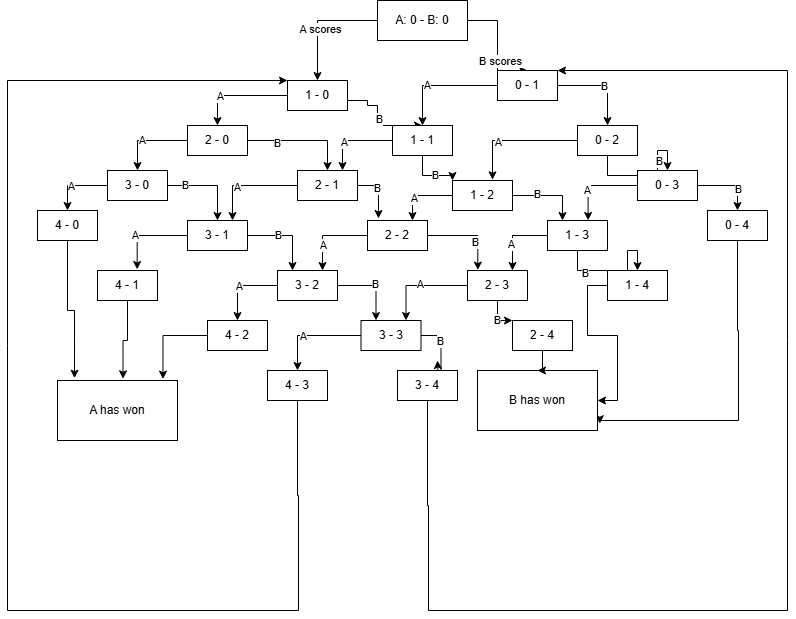
\includegraphics[width=0.5\textwidth]{ex4.png}
		\caption{ex4}
		\label{fig:ex4}
	\end{figure}
\end{solution}

\question \textbf{Bus performance analysis exercise} \\ 
In a computer system, three types of buses are commonly used: 

\begin{itemize}
    \item \textbf{Data Bus}: Transfers actual data between components (e.g., CPU and memory).
    \item \textbf{Address Bus}: Carries the address of the memory location or I/O device being accessed.
    \item \textbf{Control Bus}: Carries control signals (e.g., read/write operations).
\end{itemize}

Consider a system with the following specifications:

\begin{itemize}
    \item \textbf{Data Bus Width}: 16 bits.
    \item \textbf{Address Bus Width}: 16 bits.
    \item \textbf{Control Bus Width}: 2 bits.
    \item Each bus has the same transfer rate, and each data transfer takes 10 clock cycles.
    \item \textbf{Clock Speed}: 50 MHz.
\end{itemize}

\begin{enumerate}[label=\arabic*.]
    \item \textbf{Calculate the data transfer rate (in bytes per second) of the data bus.}

    \item \textbf{Determine how long it will take to read 10 MB (megabytes) of data from memory using the data, address, and control buses, assuming:}
    \begin{itemize}
        \item The address and control buses transfer addresses and control signals only once per data transfer.
        \item Ignore memory access delays.
    \end{itemize}
\end{enumerate} \qpoints{15}

\begin{solution}
    \begin{itemize}
        \item data-bus transfers per second: $50 MHz /(10 cycles/transfer) = 5*10^6$
        Bytes transferred per second $= 5 * 10^6 transfers/s * 2 bytes/transfer = 10 * 10^6 bytes$ so 10 $MB/s$
		\item each cycle = 20 ns, so 30 cycles = 30*20 ns = 600 ns 30 * 20 ns = 600 ns per 2 bytes.
		\item $we have (10*10^6)/2 = 5 * 10 ^6 transfers so total time = 5 * 10^6 transfers * 600 ns/transfer = 3*10^9ns = 3s.$
    \end{itemize}
\end{solution}

\question \textbf{Cache Performance Comparison} \begin{itemize}
    \item \textbf{Cache size}: 64 KB
    \item \textbf{Cache block size}: 32 bytes
    \item \textbf{Cache access time}: 2 nanoseconds
    \item \textbf{Memory access time}: 50 nanoseconds
    \item The system cache is \textbf{direct-mapped}, and the CPU generates \textbf{32-bit memory addresses}. 
    \item The cache has a \textbf{hit ratio of 85\%}.
\end{itemize}

The CPU reads 10 MB of data from memory in a random access pattern, first checking the cache. If the data is not found in the cache, it is retrieved from memory.

\begin{enumerate}[label=\arabic*.]
    \item Calculate the total time required to read the data with the given hit ratio.
    \item Determine the time required to read the same data without using the cache.    
    \item Compare the performance with and without the cache. Express the improvement as a percentage.
\end{enumerate} \qpoints{15}

\begin{solution}
	\begin{itemize}
    \item average access time per byte $= (0,85 * 2 ns) + (0,15 * 50 ns) = 1.7 ns + 7.5 ns = 9.2 ns. Total time = 10^7 bytes * 9,2 ns/byte = 9.2 * 10^7 ns = 0.092 s.$
    \item every access goes to memory at 50 ns per byte, so total time is: $10^7 * 50 = 5 * 10^8 = 0.5 s.$
    \item speedup = 0.5/0.092 = 5.43 (approximately). imporovement = (no-cache time - cache time)/ (no-cache time) * 100\% = (0.5-0.092)/0.5 * 100\% = 81.6 (approximately)
\end{itemize}
\end{solution}

\question Consider a processor with a 4-stage pipeline (Fetch, Decode, Execute, Write-back).  Each stage takes 10 nanoseconds to complete. Assume the following without  pipelining, a single instruction takes 40 nanoseconds to complete (10 nanoseconds for each stage) \qpoints{10}

\begin{itemize}
    \item Calculate the total time to execute 100 instructions with and without pipelining.
    \item Determine the speedup achieved using pipelining.
\end{itemize}

\begin{solution}
    \begin{itemize}
		\item without pipelining: Each instruction $= 4 stages * 10 ns/stage = 40 ns/instruction. For 100 instructions = 100*40 ns = 4000 ns = 4 microseconds$ \\
		with pipelining: (pipeline depth + N - 1) * (stage time) = 30 ns + (100 - 1) * 10 ns = 40 ns + 990 ns = 1030 ns.
		\item speedup: time without pipelining/ time with pipelining = 4000/1030 = 3.88 (approximately)
	\end{itemize}
\end{solution}



\end{questions}
\end{document}



